\documentclass{article}
\usepackage[utf8]{inputenc}
\usepackage[ngerman]{babel}
\usepackage{geometry}
\usepackage{hyperref}
\geometry{
    a4paper,
    left=3cm,
    right=2cm,
    top=3cm,
    bottom=3cm
}

\usepackage{graphicx}

\usepackage{tikz}
\usetikzlibrary{positioning}

\usepackage{parskip} 
\setlength{\parindent}{0pt} % Set horizontal indent between paragraphs
\setlength{\parskip}{5pt} % Set vertical spacing between paragraphs

\title{Kilter-Grade-Estimator}
\author{Pascal Lüscher}
\date{}

\begin{document}

\maketitle

\begin{minipage}[t]{0.45\textwidth}
    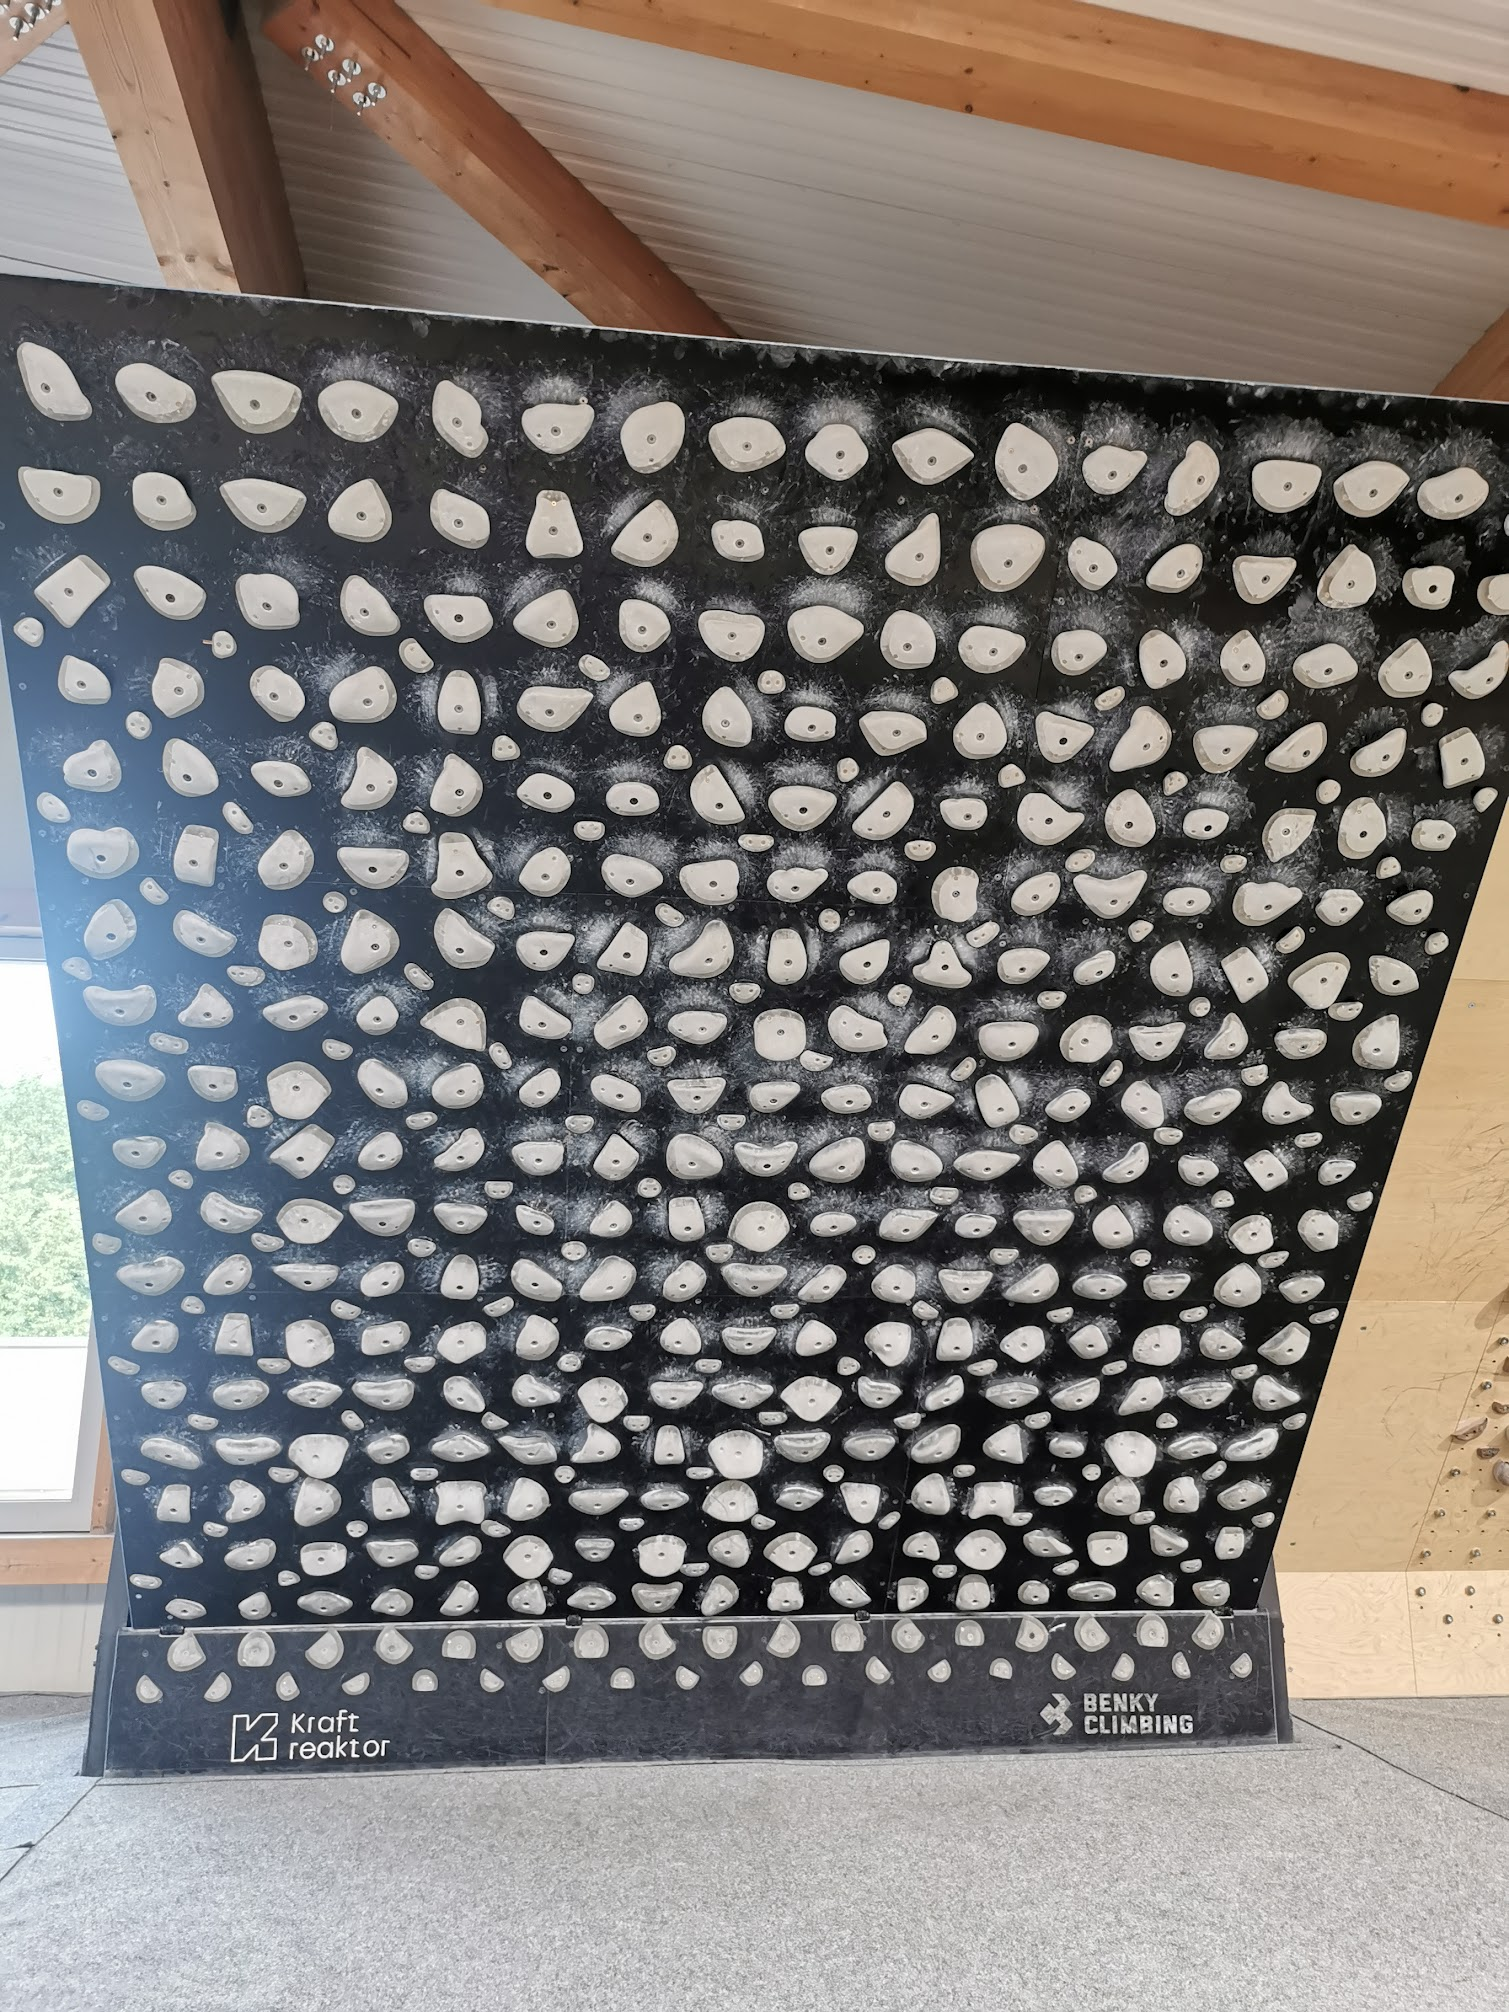
\includegraphics[width=.8\textwidth]{./media/Kilter_Board.jpg}    
\end{minipage}
\hfill
% Second minipage
\begin{minipage}[t]{0.45\textwidth}
    \resizebox{\textwidth}{!}{\begin{tikzpicture}[shorten >=1pt,->,draw=black!50, node distance=\layersep]
    \tikzstyle{every pin edge}=[<-,shorten <=1pt]
    \tikzstyle{neuron}=[circle,fill=black!25,minimum size=17pt,inner sep=0pt]
    \tikzstyle{input neuron}=[neuron, fill=green!50];
    \tikzstyle{output neuron}=[neuron, fill=red!50];
    \tikzstyle{hidden neuron}=[neuron, fill=blue!50];
    \tikzstyle{annot} = [text width=4em, text centered]

    \newcommand{\layersep}{2.5cm}

    % Draw the input layer nodes
    \foreach \name / \y in {1,...,7}
        \node[input neuron, pin=left:Input] (I-\name) at (0,-\y cm) {};

    % Draw the hidden layer 1 nodes
    \foreach \name / \y in {1,...,5}
        \path[yshift=-1cm]
            node[hidden neuron] (H1-\name) at (\layersep,-\y cm) {};

    % Draw the hidden layer 2 nodes
    \foreach \name / \y in {1,...,4}
        \path[yshift=-1.5cm]
            node[hidden neuron] (H2-\name) at (2*\layersep,-\y cm) {};

    % Draw the hidden layer 3 nodes
    \foreach \name / \y in {1,...,3}
        \path[yshift=-2cm]
            node[hidden neuron] (H3-\name) at (3*\layersep,-\y cm) {};

    % Draw the output layer nodes
    \foreach \name / \y in {1,...,1}
        \path[yshift=-3cm]
            node[output neuron, pin={[pin edge={->}]right:Output}] (O-\name) at (4*\layersep,-\y cm) {};

    % Connect every node in the input layer with every node in the
    % hidden layer 1
    \foreach \source in {1,...,7}
        \foreach \dest in {1,...,5}
            \path (I-\source) edge (H1-\dest);

    % Connect every node in hidden layer 1 with every node in hidden
    % layer 2
    \foreach \source in {1,...,5}
        \foreach \dest in {1,...,4}
            \path (H1-\source) edge (H2-\dest);

    % Connect every node in hidden layer 2 with every node in hidden
    % layer 3
    \foreach \source in {1,...,4}
        \foreach \dest in {1,...,3}
            \path (H2-\source) edge (H3-\dest);

    % Connect every node in hidden layer 3 with every node in output
    % layer
    \foreach \source in {1,...,3}
        \foreach \dest in {1}
            \path (H3-\source) edge (O-\dest);

    % Annotate the layers
    \node[annot,above of=H1-1, node distance=1cm] (hl1) {Hidden layer 1 (512)};
    \node[annot,above of=H2-1] {Hidden layer 2 (256)};
    \node[annot,above of=H3-1] {Hidden layer 3 (128)};
    \node[annot,above of=I-1] {Input layer (around 1200)};
    \node[annot,above of=O-1] {Output layer (1)};
\end{tikzpicture}}
\end{minipage}



Dieses Projekt zielt darauf ab, ein Modell zur Schätzung der Schwierigkeitsgrade von Kletterrouten auf einem Kilterboard zu entwickeln.
Dabei werden Daten aus einer SQLite-Datenbank der Kilterboard-App genutzt.
Der Datensatz umfasst über 200.000 Routen mit Merkmalen wie Griffplatzierungen und verschiedenen Kletterwinkeln. 
Die Analyse umfasst die Datenbereinigung, One-Hot-Encoding der Griffplatzierungen und die Erstellung von Modellen mittels 

\begin{itemize}
\item logistischer Regression
\item linearer Regression
\item XGBoost
\item neuronalen Netzen
\end{itemize}

Erste Modelle zeigten eine begrenzte Genauigkeit, was zu einer weiteren Untersuchung der Datenqualität und einer Vereinfachung der Schwierigkeitskategorien führte.
Letztendlich erbrachte ein neuronales Netzwerk, das mit gefilterten, qualitativ hochwertigeren Daten trainiert wurde,
die vielversprechendsten Ergebnisse. 
Es erzielte einen MAE von 1,29 für die ursprünglichen Daten und 0,81 für vereinfachte Schwierigkeitskategorien,
wodurch die Kletterschwierigkeit innerhalb akzeptabler Grenzen effektiv vorhergesagt werden konnte.

Für zukünftige Projekte empfehle ich, die Griffarten der Kletterrouten stärker zu berücksichtigen,
da dies die Leistung des Modells verbessern könnte. 
Des Weiteren bietet sich die Möglichkeit, weitere neuronale Netzwerkarchitekturen zu erforschen und zu evaluieren,
 um die Vorhersagegenauigkeit weiter zu steigern.

Für weitere Infos: \href{https://github.com/Isitar}{Github Profile (Isitar)}

\end{document}